\documentclass[a4paper]{article}
\usepackage[utf8]{inputenc}
\usepackage[english,italian]{babel}
\usepackage{afterpage}
\usepackage{graphicx}
\usepackage{fancyvrb}
\usepackage[inline]{enumitem}

\title{RELAZIONE PROGETTO\\PROGRAMMAZIONE ad OGGETTI}
\author{Nicola Dalla Costa (1051222)}
\date{}

\begin{document}
\maketitle
%\afterpage{\null\thispagestyle{empty}\clearpage}
\raggedbottom

\section*{Introduzione}
Lo scopo del progetto, denominato \textit{LinQedIn}, era lo sviluppo in C++/Qt di un sistema minimale per l'amministrazione ed utilizzo tramite interfaccia utente grafica di un (piccolo) database di contatti professionali ispirato a LinkedIn. 

LinkedIn è il principale servizio web di rete sociale per contatti professionali, gratuito ma con servizi opzionali a pagamento. Attualmente prevede quattro tipologie di account, ma per semplicità sono state considerate solo Business ed Exectutive, oltre a quella gratuita Basic.

Tra le funzionalità disponibili all'utente amministratore troviamo: inserimento e rimozione utenti, ricerca utenti e cambio tipologia di account di un utente. Lato utente invece sono disponibili: aggiornamento informazioni profilo, aggiunta e rimozione contatti ed una funzionalità di ricerca crescenti in base alla tipologia di account.

Per la realizzazione della GUI è stato utilizzato IDE QtCreator ma senza l'ausilio del tool QtDesigner. In questo modo il codice risulta più pulito.

Nonostante il progetto si limiti ad offrire le funzionalità richieste, nella realizzazione è stata data molta importanza a concetti come information hiding, modularità, estendibilità e qualità del codice.

La realizzazione del progetto è costata solo nell'ultimo mese di lavoro più di 100 ore. Impossibile definire una quantità totale indicativa.

La presente relazione non deve essere considerata come documentazione. Viene fornita una breve descrizione di tutte le classi e della logica, soffermandosi solo nei dettagli più importanti.\footnote{Una documentazione più dettagliata è presente nel codice sottoforma di commenti.}

\section*{Parte Logica}
La parte logica si compone di 16 classi che ora vederemo nel dettaglio.

\subsection*{Profilo}
Utilizzata per la gestione delle informazioni personali di un utente. Di queste informazioni fanno parte: nome, cognome, data di nascita e stato civile. 

La rappesentazione interna viene nascosta con l'utilizzo di un puntatore ad una classe interna privata InfoPersonali. In questo modo viene nascosto all'utente finale la modalità di memorizzazione dei dati (\textit{information hiding}).

L'utilizzo di un puntatore per nascondere la rappresentazione interna può provocare problemi di condivisione di memoria. Per questo motivo in caso di costruzione di copia di un oggetto Profilo, viene effettuata una copia profonda del campo dati di tipo InfoPersonali*. In questi casi è necessario che anche l'operatore di assegnazione sia ridefinito in modo che effettui un'assegnazione profonda. Vengono forniti metodi getter e setter per tutte le informazioni memorizzabili in un oggetto Profilo.\footnote{Per questa e tutte le altre classi seguenti saranno omessi i metodi getter e setter.}

\subsection*{Rete}
Utilizzata per la gestione della lista dei contatti di un utente. I contatti sono memorizzati come oggetti di tipo SmartUtente che saranno descritti più avanti.

La rappresentazione interna viene nascosta con l'utilizzo di un puntatore ad una classe interna privata Rete\_rapp. A differenza del campo dati di tipo InfoPersonali* per il Profilo, qui si è pensato di gestire la copia di oggetti Rete con la tecnica del \textit{references counting}: in caso di copia o distruzione di un oggetto Rete si limita ad incrementare o diminuire il campo riferimenti. La distruzione effettiva si verifica solo quando il campo riferimenti arriva a 0.

Per ottenere la lista dei contatti, poichè non è nota la modalità di memorizzazione, è stato fornito il metodo \texttt{QVector<SmartUtente> getContactsList() const} che ritorna la lista dei contatti in un semplice QVector. Oltre ai metodi per aggiungere e rimovere un contatto, viene reso disponibile il metodo \texttt{bool isContact() const} che controlla la presenza di un utente nella lista dei contatti.

\subsection*{Lavoro e Titolo}
Utilizzate per la gestione delle esperienze lavorative e dei titoli di studio rispettivamente. La prima memorizza informazioni riguardo: nome dell'azienda, ruolo o posizione ricoperta, data di inizio e di fine. La seconda memorizza informazioni riguardo: nome della scuola o università, data di conseguimento diploma o laurea e campo di studi.

Sono inoltre fornite le due classi \textbf{SmartLavoro} e \textbf{SmartTitolo}, le quali permettono di gestire in modo automatico il campo riferimenti in caso di condivisione di memoria tra puntatori ad oggetti di tipo Lavoro o Titolo.

\subsection*{Esperienza e Formazione}
Utilizzate per memorizzare la lista delle esperienze lavorative e per la lista dei titoli di studio di un utente. Le esperienze lavorative vengono memorizzate con puntatori ad oggetti di tipo Lavoro. I titoli di studio vengono memorizzati come puntatori ad oggetti di tipo Titolo.

Come per la classe Rete, la rappresentazione interna viene nascosta con l'utilizzo di puntatori alle classi interne private Esperienza\_rapp e Formazione\_rapp definite in Esperienze e Formazione rispettivamente. La copia degli oggetti viene sempre gestita con la tecnica del references counting e sono disponibili dei metodi che ritornano le liste delle esperienze lavorative e dei titoli di studio come istanze di QVector.

Per entrambe è stato inoltre fornito un iteratore con i soli metodi \texttt{begin()}, \texttt{hasNext()} e \texttt{next()}. La realizzazione di questi iteratori è stata difficile in quanto le classi interne possono accedere solo ai membri statici delle classi contenitrici ed entrambe le classi (contenitrice ed iteratore) dovevano rispettare l'information hiding.

\subsection*{Utente}
Utilizzata per la gestione degli utenti del client. Contiene un campo dati di tipo QString per memorizzare l'username, un campo dati Profilo e tre campi dati puntatore ad oggetti di tipo Rete, Formazione ed Esperienza. 

La scelta dei puntatori è dovuta al fatto che le liste di contatti, esperienze lavorative e titoli di studio possono crescere e la copia di utenti potrebbe comportare spreco di memoria. La copia degli utenti viene sempre gestita con la tecnica del references counting.

Fornire metodi che permettono un accesso diretto ad un campo dati tramite puntatore non è una buona pratica. Per questo motivo sono stati riportati tutti i metodi pubblici dei campi dati puntatore nella classe Utente, i quali invocano i metodi corrispondenti nella classe di appartenenza. Purtroppo in questo modo si crea una forte dipendenza con le classi Rete, Formazione ed Esperienza ma l'utilizzo dei metodi risulta più semplice.

Viene fornita inoltre la classe \textbf{SmartUtente} per la gestione automatica del campo riferimenti in caso di condivisione di memoria tra puntatori ad oggetti di tipo Utente.

\subsubsection*{Gerarchia}
La classe Utente è una classe base polimorfa ed astratta in quanto contiene il distruttore definito virtuale e puro (condizione necessaria e sufficiente ma anche altr metodi sono dichiarati virtuali o virtuali puri).

Inizialmente, poichè la differenza principale tra le varie tipologie di account sta nell'essere gratuito o meno, erano state create due sottoclassi (sempre astratte) UtenteGratis e UtentePagante. Da UtenteGratis poi veniva derivata la classe concreta \textbf{UtenteBasic}, mentre da UtentePagante venivano derivate le classi \textbf{UtenteExecutive} ed \textbf{UtenteBusiness}.

Nonostante questa fosse la gerarchia più corretta, data l'assenza di nuovi campi dati o metodi definiti nelle due classi intermedie (e per semplicità), è stato deciso di rimuovere UtentePagante ed UtenteGratis e far derivare direttamente le 3 classi concrete da Utente.

\subsubsection*{Ricerca}
La funzionalità di ricerca è stata l'ultima ad essere sviluppata. Purtroppo la versione definitiva non è una buona soluzione ma non lo erano nemmeno le altre valutate e provate.

Una delle versioni faceva uso della classe FuntoreRicerca, classe funtore, definita interna ad Utente e di un metodo \texttt{QVector<SmartUtente> searchUsers( QVector<SmartUtente> )} virtuale puro che in base alla ridefinizione nelle classi concrete ritornava un vettore di nuovi oggetti SmartUtente creati di copia dal vettore passato come parametro, ai quali venivano rimossi i campi non visualizzabili in base alla tipologia. 

Questo però aveva comportato la necessità di aggiungere dei metodi \texttt{*clone() const} e di costruttori appositi in tutte le classi concrete della gerarchia Utente e lo stesso nelle classi Rete, Formazione ed Esperienza, la ridefinizione dell'operatore \texttt{delete} nelle ultime 3 e l'aggiunta di metodi per distruggere manualmente i campi dati puntatore della classe Utente in base alle informazioni che si volevano rendere disponibili. In questo modo però era necessaria anche la modifica dei metodi della classe Utente per controllare che i campi dati puntatore fossero validi. La necessità di distruggere i campi dati era dovuta al fatto che, ad esempio, una lista di contatti vuota è diversa da una lista di contatti inaccessibile.

Anche se funzionante come soluzione era troppo complessa e c'era il serio rischio di introduzione di errori. Per questo motivo si è passati ad una soluzione molto più semplice. Tolti tutti i metodi, costruttori ed operatori aggiunti e la classe funtore, si è aggiunto un metodo virtuale puro \texttt{QList<QString> getUserInfo() const} che restituisce una lista con degli indicatori per i campi accessibili dall'utente. Purtroppo anche se più semplice per molti versi è peggiore della precedente in quanto in questo modo il risultato non è l'utente con le sole informazioni visualizzabili, ma una semplice lista da utilizzare per filtrarle.

Durante la stesura di questa relazione mi sono reso conto che la prima soluzione funzionante era la migliore e la complessità era dovuta al fatto che i campi dati puntatore venivano creati con una lista di default, mentre la cosa più logica era quella di inizializzare i campi a 0 ed aggiungere i controlli necessari nei metodi in Utente.

\subsection*{Database}
Utilizzata per la gestione degli utenti del client. Si è deciso di memorizzare gli utenti nel database tramite una mappa, dove l'username è la chiave associata allo SmartUtente (puntatore ad Utente). La rappresentazione interna è nascosta all'utente finale tramite l'utilizzo della classe interna Database\_rapp. In questo modo il codice è indipendente dalla rappresentazione e possono essere effettuate modifiche alla modalità di memorizzazione senza aver bisogno di modificare i metodi forniti all'utente. Altro motivo è dovuto al fatto che le funzioni di ricerca, inserimento e rimozione di un utente viene fatta in tempo O(1), quindi costante.

La dichiarazione di amicizia con la classe LinQedInAdmin è necessaria in quanto i metodi, dichiarati privati, per l'inserimento e rimozione di utenti da database deve essere disponibile solo all'utente amministratore.

Il salvataggio di utenti avviene su file XML con l'utilizzo di QXmlStreamWriter, mentre il caricamento con QXmlStreamReader. In caso il file non esista viene creato. Particolare attenzione bisogna dare al caricamento degli utenti, in quanto la creazione della lista dei contatti avviene solo dopo aver caricato tutti gli utenti nel database. Questo perchè la lista dei contatti è composta da oggetti SmartUtente e non si può inserire un utente se non esiste.

Tra gli altri metodi pubblici, viene fornito il metodo \texttt{QVector<SmartUtente> getUsersList() const} che restituisce la lista degli utenti del database.

\subsection*{LinQedInClient}
Utilizzata per la gesione del client lato utente. Contiente un campo dati SmartUtente che corrisponde all'utente utilizzatore del client ed un puntatore ad un oggetto Database che rappresenta il database degli utenti del client. Mette a disposizione dei semplici metodi per salvare i campi dati dell'utente utilizzatore del client. La definizione di questi metodi si limita a richiamare la funzione \texttt{void saveUsersList() const} in quanto, essendo un piccolo database di utenti, la riscrittura di tutto il file non è onerosa.

\subsection*{LinQedInAdmin}
Utilizzata per la gestione del client lato amministratore. A differenza di LinQedInClient, questa classe funziona come controller (del pattern Model-View-Controller) in quanto i metodi forniti collegano la parte logica alle funzionalità della parte grafica. Vengono messi a disposizione metodi per inserimento, rimozione, ricerca e cambio tipolgia di account degli utenti, oltre ai metodi per il caricamento ed il salvataggio.

\section*{Parte Grafica}
La parte grafica si compone di 29 classi. Nella realizzazione della GUI si è cercato di seguire i principi del \textit{Material Design}.

Una delle caratteristiche che accomunano tutte la componenti della GUI è la presenza dei due metodi privati ausiliari \texttt{void initUI()} e \texttt{void setupUI()} per l'inizialiazzazione e realizzazione della GUI rispettivamente. Inoltre la ridefinizione del distruttore non è necessaria in quanto nell'inizializzazione dei campi dati di tipo puntatore viene passato come QWidget parent \texttt{this}. In questo modo alla distruzione del parent (quindi dell'instaza della classe) vengono distrutti tutti gli oggetti figli.

\subsection*{LinQedInWindow}
Classe base astratta che estende QMainWindow, da utilizzare come classe base per tutte le finestre del client. Offre campi e metodi comuni. Così facendo la necessità di una stessa modifica in ognuna di queste può essere effettuata una sola volta. Le classi derivate sono: LoginWindow, AdminWindow e ClientWindow.

\subsection*{LinQedInDialog}
Classe base astratta che estende QDialog, da utilizzare come classe base per tutte le finestre di dialogo del client. Come per LinQedInWindow, offre campi e metodi comuni. Le classi derivate sono: AddJobDialog, AddTitleDialog, AddUserDialog, AdminLoginDialog, AdminSearchDialog, ChangeUserTypeDialog, EditJobDialog, EditProfileDialog e EditTitleDialog.

\subsection*{LoginWindow}
\begin{figure}[!ht]
\centering
\caption{Finestra di login}
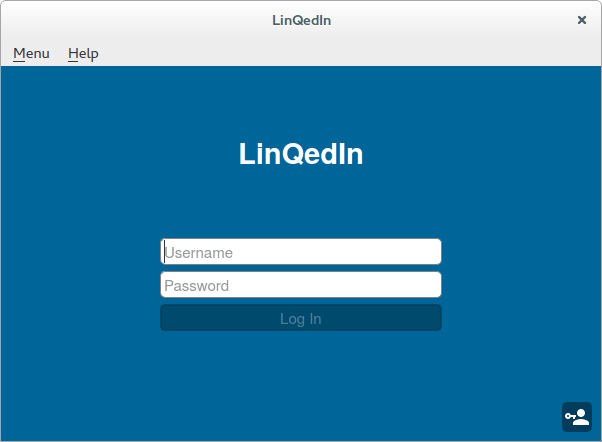
\includegraphics[width=0.6\textwidth]{LoginWindow.png}
\end{figure}

L'accesso ad entrambi i client (per gli utenti o per l'amministratore) avviene tramite la stessa finestra di login.

Il pulsante per l'accesso utente risulta disabilitato e viene abilitato solo quando entrabi i campi (username e password) risultano non vuoti. Per fare questo è stato connesso lo slot \texttt{void checkInput( QString )} al segnale \texttt{textChanged( QString )} che viene emesso ogni volta che il contenuto di uno tra i due oggetti QLineEdit viene modificato. Gli spazi ad inizio e fine vengono ignorati. Il controllo effettivo avviene solo nell'username, mentre il campo password è stato aggiunto solo per completezza. Il controllo di entrambi i campi non è stato ritenuto molto importante, ma è stata data più attenzione all'utilizzo corretto delle librerie Qt, alla qualità ed all'usabilità. Non è esclusa una probabile implementazione futura.

Al pulsante di log in è connesso lo slot \texttt{void loginUser()} che crea un'istanza di ClientWindow (passando l'username) con parent 0 (quindi top-level) e distrugge l'istanza di LoginWindow.

L'accesso amministrativo avviene tramite l'apertura della finestra di dialogo di tipo AdminLoginDialog. Alla pressione del pulsante nell'angolo in basso a destra è connesso lo slot \texttt{void openAdminLoginDialog()} che crea un oggetto AdminLoginDialog.

\begin{figure}[!ht]
\centering
\caption{AdminLoginDialog}
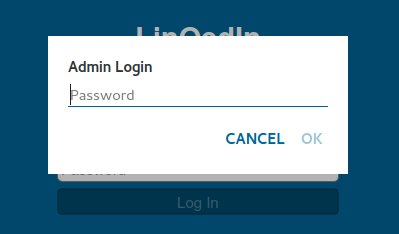
\includegraphics[width=0.4\textwidth]{AdminLoginDialog.png}
\end{figure}

Nella costruzione di quest'ultima viene passato come oggetto QWidget parent l'istanza della classe LoginWindow. In questo modo non risulta possibile chiudere il client senza prima aver chiuso la finestra di dialogo.

Come per l'accesso utente, il pulsante di conferma password risulta disabilitato finchè la password inserita contiene almeno un carattere. Gli spazi ad inizio e fine sono esclusi. Al pulsante di conferma è connesso lo slot \texttt{void checkPassword()} (per semplicità, anche in questo caso non avviene una verifica effettiva) che prima chiude la finestra di login e successivamente emette il segnale \texttt{void adminLoginSignal()}. Al segnale è connesso lo slot \texttt{void adminLogin()} del parent che si comporta come lo slot per l'accesso utente ma questa volta crea un'istanza di AdminWindow.

\subsection*{ClientWindow}
Nella realizzazione della GUI della classe ClientWindow mi sono ispirato ad un concept presente su \textit{Behance}\footnote{\textit{Linkedin Material Design}, realizzato da Rico Monteiro e pubblicato con licenza ``Attribution-NonCommercial 3.0 Unported (CC BY-NC 3.0)''}.

\begin{figure}[!ht]
\centering
\caption{ClientWindow}
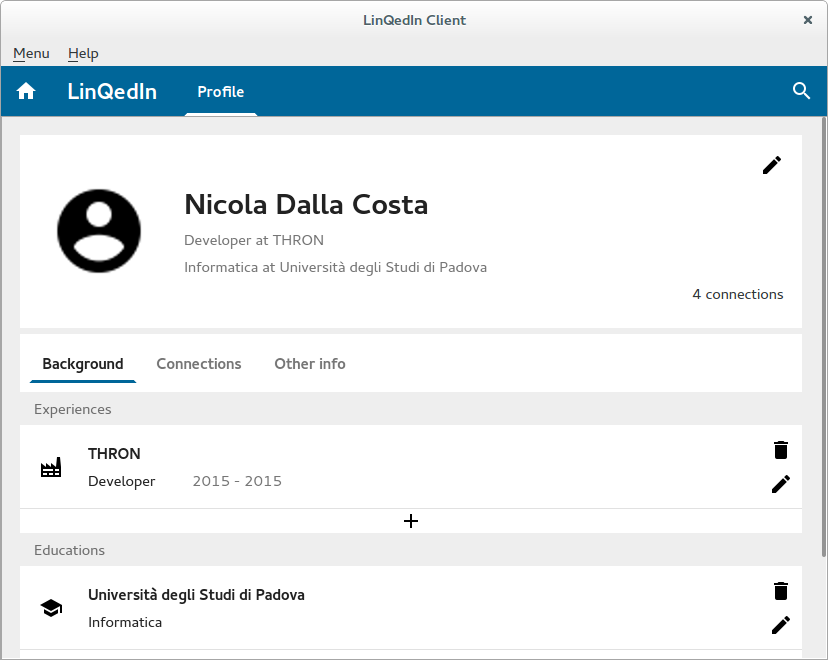
\includegraphics[width=0.7\textwidth]{ClientWindow.png}
\end{figure}

\end{document}